\iffalse
\documentclass[journal,12pt,twocolumn]{IEEEtran}
\usepackage{graphicx}
\graphicspath{{./figs/}}{}
\usepackage{amsmath,amssymb,amsfonts,amsthm}
\newcommand{\myvec}[1]{\ensuremath{\begin{pmatrix}#1\end{pmatrix}}}

\let\vec\mathbf

\title{
Matrix-Lines
}
\author{Kukunuri Sampath Govardhan}
\begin{document}
\maketitle
\tableofcontents
\bigskip
\section{Problem Statement}
\fi
Find equation of a line passing trough a point (2,2) and cutting off intercepts on the axes whose sum is 9.
	\begin{figure}[!ht]
		\centering
 \includegraphics[width=\columnwidth]{chapters/11/10/2/13/figs/assign4.png}
		\caption{}
		\label{fig:11/10/2/13}
  	\end{figure}
	\\
	\solution 
\iffalse
\section{Construction}
\begin{figure}[h]
    \centering
\includegraphics[width=\columnwidth]{figs/assign4.png}
    \caption{Equation of the Straight Line}
    \label{fig:my_label}
\end{figure}
\vspace{2cm}
\begin{table}[h]
    \centering
    \begin{tabular}{|c|c|c|}
       \hline
       \textbf{Symbol}&\textbf{Value}&\textbf{Description}  \\
       \hline
	    $\vec{P}$ & $\myvec{
		    a\\
		    0}$
	    & Point on X-axis\\
        \hline
	    $\vec{Q}$ & $\myvec{0\\b}$
 & Point on Y-axis\\
        \hline
	    $\vec{R}$ & $\myvec{
  2\\
  2}$
 & Given Point \\
        \hline
        a + b & 9 & Given Condition\\
        \hline
    \end{tabular}
    \caption{Parameters}
    \label{tab:my_label}
\end{table}


\section{Solution}
Given that resultant line passes through point(2,2) and intercepts on axes whose sum is 9 (
\fi
Let the $x$ intercept be $a$ and the $y$ intercept be $b$. 
Then 
\begin{align}
		\label{eq:11/10/2/13-a+b}
 a + b = 9
\end{align}
Let 
\begin{align}
{\vec{P}}=\myvec{
  a\\
  0}
 , {\vec{Q}}=\myvec{
  0\\
  b}
  , {\vec{R}}=\myvec{
  2\\
  2}
\end{align}
Since the points are collinear, from 
	\eqref{eq:normal_line-collinear},
	we obtain the matrix
\begin{align}
	\myvec{ \vec{P}-\vec{Q} &\vec{P}-\vec{R}} 
	=
	 \myvec{
  a & a-2\\
  -b & -2
 }
\end{align}
which is singular if the determinant
\begin{align}
	-2a +b(a-2) = ab -2\brak{a+b} = 0
\end{align}
yielding
\begin{align}
	ab = 18
		\label{eq:11/10/2/13-ab}
\end{align}
upon substituting from 
		\eqref{eq:11/10/2/13-a+b}.
		\eqref{eq:11/10/2/13-ab}
		and 
		\eqref{eq:11/10/2/13-a+b}
		form
\begin{align}
	x^2 -9x +18 = 0
\end{align}
with roots
\begin{align}
	x = 6,3
	\\
	\text{or, }
	\myvec{a \\ b} = \myvec{6 \\ 3}, \myvec{3\\6}
\end{align}
Since the direction vector of the line is 
\begin{align}
	\vec{P}-\vec{Q} = \myvec{a \\ -b},
\end{align}
the normal vector is 
\begin{align}
	\vec{n} = \myvec{b \\ a} \equiv \myvec{1 \\ 2}, \myvec{2\\1}
\end{align}
Thus, the possible equations of the line are 
\begin{align}
\myvec{1 & 2}\vec{x} = 6
	\\
	\myvec{2&1}\vec{x} = 6
\end{align}
\iffalse
\\
\\
Equation of line is ${\vec{n^{\top}}\vec{X}} = c$.\\
\\
Now we have 3 points which lies on same line so,\\
 The Equation of line through ${\vec{P}}$ is\\
 Hence, 
\begin{align}
	\vec{n}^{\top}
	\myvec{
  a\\
  0}
  &= c 
\\
	\vec{n}^{\top}
     \myvec{
  0\\
  b
 }
	&= c 
  \\
  \implies 
	\vec{n}^{\top}
	\myvec{
  a\\
  b
}
	&= 2c 
\end{align}
upon addition.
Also, 
\begin{align}
	\vec{n}^{\top}
	\myvec{
  2\\
  2}
  = c 
\end{align}
	Thus, we obtain, upon clubbing the above two equations,
 \begin{align}
	 \vec{n}^{\top}
	 \myvec{
  a & 9-a\\
  2 & 2
 }
	 = c\myvec{
  2\\
  1}
\end{align}
yielding
 \begin{align}
	 \vec{n^{\top}} &= 
	 \myvec{
  a & 9-a\\
  2 & 2
 }
  ^{-1}
	 \myvec{
  2\\
  1}
 c 
\end{align}
%
  \\
  Thus, we get \textbf{a = 2, b = 9-a = 7}\\
  \\
  by substuting a in eq6, finally\\
  \\
   \begin{align}
	   \vec{n^{\top}} = 
	   \myvec{
  0.3\\
  0.2}
 .c
 \end{align}
  \\
The Resultant Equation of line is ${\vec{n^{\top}}\vec{X}} = c$ \\
\\
 \begin{align}
	 \myvec{
  0.3\\
  0.2\\
 }
	 .\vec{X}.c = c
 \end{align}
  \\
i.e,    \\
\begin{align}
	\myvec{
  3\\
  2}
	.\vec{X} = 10
 \end{align}
\\
\textbf{
Therefore equation of the line is, \\
\begin{align}
	\myvec{
  3\\
  2}
	. \vec{X} = 10
 \end{align}}
\begin{center}
    \textbf{3x + 2y = 10}
\end{center}
\section{Software}
Download the following code using,
\begin{table}[h]
    \centering
    \begin{tabular}{|c|}
    \hline \\
         svn co https://github.com/\\mygit-sampath-govardhan/fwc-iith-assignments/blob/\\5b65abbf8e5e3c803b1bff8cf4a95092e100de75/\\Assignment-4(Matrices-line)/codes/Assignment4.py  \\
         \\
\hline
    \end{tabular}
\end{table}
\\
and execute the code by using command
\begin{center}
\textbf{Python3  Assignment4.py}\\
\end{center}

\section{Conclusion}
We found the equation of a line passing trough a point
(2,2) and cutting off intercepts on the axes whose
sum is 9.

\end{document}
\fi
